\documentclass{beamer}
\usepackage{amsfonts,amsmath,oldgerm}
\usetheme{sintef}
\usepackage{xeCJK}
\usepackage{booktabs}
\usepackage{array}
\usepackage{tikz}
\usetikzlibrary{positioning,arrows.meta,shapes.geometric}

% ---- 中文字体（Windows 自带，避免回退到 Fandol）----
\setCJKmainfont{Microsoft YaHei}
\setCJKsansfont{Microsoft YaHei}
\setCJKmonofont{SimHei}

\newcommand{\testcolor}[1]{\colorbox{#1}{\textcolor{#1}{test}}~\texttt{#1}}
\usefonttheme[onlymath]{serif}
\titlebackground*{assets/background}

\newcommand{\hrefcol}[2]{\textcolor{cyan}{\href{#1}{#2}}}
\newcommand{\good}{\textcolor{sintefgreen}{$\bullet$}}
\newcommand{\warn}{\textcolor{sintefyellow}{$\bullet$}}
\newcommand{\bad}{\textcolor{sinteflilla}{$\bullet$}}

\title{函数漏洞检测智能体工具}
\subtitle{课程项目中期汇报}
\author{组长：李柏谚\quad 组员：杨聃、王义卓、孙伊凡、徐培栋}
\date{2026 年 11 月\quad 高级软件工程}

\begin{document}
\maketitle

% ============================================================ 目录
\footlinecolor{sintefgreen}
\begin{frame}{汇报提纲}
\framesubtitle{基本信息 → 方案与设计 → 进展与结果 → 问题与计划}
\small
\begin{columns}[t]
\begin{column}{0.48\textwidth}
\begin{itemize}
  \item \textbf{01\quad 项目基本信息}
  \item[$\;$] 代码库、团队分工、计划与进度
  \item \textbf{02\quad 项目意义与目标}
  \item[$\;$] 要解决什么问题、做到什么程度
  \item \textbf{03\quad 技术方案}
  \item[$\;$] 技术栈、关键算法、系统架构
  \item \textbf{04\quad 功能设计}
  \item[$\;$] 功能组成、BDD 用户故事、低保真界面
\end{itemize}
\end{column}
\begin{column}{0.48\textwidth}
\begin{itemize}
  \item \textbf{05\quad 开发进展}
  \item[$\;$] 各模块完成度与界面演示
  \item \textbf{06\quad 评测结果}
  \item[$\;$] 150 对样本的成对统计与基线对比
  \item \textbf{07\quad 创新点与特色}
  \item \textbf{08\quad 当前问题与下一步}
  \item[$\;$] 问题定位、优化措施、预期指标
\end{itemize}
\end{column}
\end{columns}
\end{frame}

% ============================================================ 01 基本信息
\begin{frame}{01 · 项目基本信息}
\framesubtitle{项目名称、代码库与团队分工}
\small
\begin{block}{项目}
\textbf{函数漏洞检测智能体工具}：输入一个 C/C++ 函数与其所在仓库的修复提交链接，
由自主 Agent 结合领域知识库（RAG）与仓库上下文挖掘，输出「判定结果 + 判定理由 + 分析记录」。
\end{block}

\footnotesize
\textbf{代码库}：\texttt{github.com/LiLisyn123/func-vuln-agent}\\[0.2em]
\textbf{协作}：Git 分支 \texttt{main} $\leftarrow$ \texttt{dev} $\leftarrow$ \texttt{feat/*}，
任务先开 Issue，合并走 PR + 至少一人 review。

\vspace{0.3em}
\scriptsize
\begin{tabular}{@{}p{0.15\textwidth}p{0.42\textwidth}p{0.34\textwidth}@{}}
\toprule
\textbf{成员} & \textbf{负责模块} & \textbf{主要产出} \\
\midrule
李柏谚（组长） & 总体架构、智能体主流程 & 架构设计、\texttt{agent/}、\texttt{pipeline}、集成 \\
杨聃 & 领域知识库与检索 & 成对案例、BM25 索引、检索渲染 \\
王义卓 & 仓库查询工具 & 版本快照、C 解析、9 个查询工具 \\
孙伊凡 & 图形界面与批量流程 & 四页面界面、实时事件渲染、批量 \\
徐培栋 & 评测、集成与文档 & 评测口径、基线实验、测试与交付文档 \\
\bottomrule
\end{tabular}
\end{frame}

% ============================================================ 01 计划与进度
\begin{frame}{01 · 开发计划与进度安排}
\framesubtitle{七周计划，目前已进入第六周的评测调优阶段}
\footnotesize
\begin{tabular}{@{}p{0.1\textwidth}p{0.42\textwidth}p{0.36\textwidth}@{}}
\toprule
\textbf{周次} & \textbf{计划产出} & \textbf{当前状态} \\
\midrule
W1--W3 & 需求与数据摸底；历史案例入库、检索可用；仓库查询工具可用
& \good\ 已完成（知识库 3891 条案例、9 个工具） \\
W4--W5 & 打通「先检索 → 再判定 → 按需读仓库」主流程；图形界面与批量
& \good\ 已完成（可现场完整演示） \\
W6 & 300 条样本批量评测与迭代调优
& \warn\ 第一轮全量已跑完（等级 C），正在调优 \\
W7 & 技术报告、系统演示、结果提交
& \bad\ 待完成（报告初稿已完成） \\
\bottomrule
\end{tabular}

\vspace{0.6em}
\begin{colorblock}[black]{sinteflightgreen}{里程碑判定}
\footnotesize
\textbf{整体完成度约 85\%}：三条红线对应的能力全部落地并已用真实模型跑通 300 条评测，
当前工作重心从「功能实现」转向「判定质量调优」与「报告撰写」。
\end{colorblock}
\end{frame}

% ============================================================ 02 意义与目标
\begin{frame}{02 · 项目意义与目标}
\framesubtitle{漏洞多到查不过来，而传统工具与大模型各缺一块}
\footnotesize
\begin{itemize}
  \item \textbf{规模失控}：2026 年前两个季度新增 CVE 逾 \alert{3.5 万} 条，人工审计跟不上；
  \item \textbf{传统工具两难}：规则少了漏报、规则宽了误报，且说不清判定依据；
  \item \textbf{大模型缺两块}：不知道具体漏洞长什么样，也不知道谁调用了这个函数。
\end{itemize}

\vspace{0.2em}
\begin{columns}[t]
\begin{column}{0.47\textwidth}
\begin{colorblock}[black]{sinteflightgreen}{难点一：缺领域知识}
\scriptsize
对策：用历史已披露的 CVE 案例构建\textbf{可检索知识库}，
让模型先看「这类代码当年怎么坏、怎么被修」，再下判断。
\end{colorblock}
\end{column}
\begin{column}{0.47\textwidth}
\begin{colorblock}[white]{sinteflilla}{难点二：孤立函数判不了}
\scriptsize
对策：给智能体装上\textbf{仓库按需取证}能力，
自己决定何时去查调用方、被调用方、宏与类型定义。
\end{colorblock}
\end{column}
\end{columns}

\vspace{0.2em}
{\scriptsize \textbf{目标}：输入一个函数 + 仓库链接，输出「有没有漏洞 —— 凭什么 —— 怎么查出来的」；
只做判断与解释，\emph{不做自动修复、不扫全仓}。}
\end{frame}

% ============================================================ 03 技术方案
\begin{frame}{03 · 实施技术方案}
\framesubtitle{成熟、可控、可复现；核心运行时零第三方依赖}
\footnotesize
\begin{tabular}{@{}p{0.17\textwidth}p{0.34\textwidth}p{0.42\textwidth}@{}}
\toprule
\textbf{环节} & \textbf{选型} & \textbf{选择理由 / 关键设计} \\
\midrule
开发语言 & Python 3.12 & 前后端与算法统一，生态完整 \\
版本控制 & Git + GitHub & 分支模型、Issue、PR，过程可追溯 \\
协作工具 & Issue 看板 + PR Review & 每项任务可追踪、每次合并有评审 \\
智能体框架 & \textbf{自研 ReAct 框架} & 零依赖、可精确控制预算/收敛/留痕；接口与 LangGraph 对齐，可替换 \\
知识检索 & \textbf{纯 Python BM25}（无向量库） & 代码检索靠标识符命中更稳；索引仅 1.3 MB，可离线复现 \\
代码解析 & \textbf{字符级 C/C++ 扫描器} & 免原生编译依赖；接口与 Tree-sitter 解耦，可平滑替换 \\
仓库快照 & GitHub codeload tarball + git 兜底 & 按提交 SHA 精确固定版本，便于版本隔离 \\
图形界面 & Streamlit & 原生支持实时刷新与文件上传 \\
底层模型 & DeepSeek（OpenAI 兼容协议） & 改 \texttt{.env} 即可换模型，业务代码零改动 \\
数据存储 & \textbf{无数据库}：本地文件缓存 & 索引（gzip+pickle）、案例语料（JSONL）、快照目录；免部署、易复现 \\
\bottomrule
\end{tabular}
\end{frame}

% ============================================================ 03 关键算法
\begin{frame}{03 · 关键理论与算法}
\framesubtitle{三个关键机制：成对案例检索、ReAct 自主取证、严格版本隔离}
\footnotesize
\begin{columns}[t]
\begin{column}{0.32\textwidth}
\begin{colorblock}[black]{sinteflightgreen}{① 成对案例 RAG}
\scriptsize
每个案例 = 同一函数的\emph{漏洞版 + 修复版} + \emph{修复要点}（difflib 抽取的新增行）。\\[0.3em]
BM25：$\text{score}=\sum_{t}\text{idf}(t)\cdot\frac{f_t(k_1+1)}{f_t+k_1(1-b+b\cdot d/\bar d)}$\\[0.2em]
（$k_1=1.5$，$b=0.75$）\\[0.3em]
实测检索 P50 \textbf{5.8 ms}。
\end{colorblock}
\end{column}
\begin{column}{0.34\textwidth}
\begin{colorblock}[black]{sintefyellow}{② ReAct 自主决策}
\scriptsize
模型在循环中自主决定：\\
· 调哪个工具（12 个只读工具）\\
· 调几次（上限 12 轮 / 20 次）\\
· 何时收口（结构化 \texttt{submit\_report}）\\[0.3em]
框架只做三件事：能力边界、预算约束、过程留痕；不预置流水线顺序。
\end{colorblock}
\end{column}
\begin{column}{0.30\textwidth}
\begin{colorblock}[white]{sintefpurple}{③ 版本隔离}
\scriptsize
\texttt{target=1} → 只取父提交\\
\texttt{target=0} → 只取提交后版本\\[0.3em]
快照按 SHA 固定、缓存复用；\\不提供 diff，提示词不含标签。
\end{colorblock}
\end{column}
\end{columns}

\vspace{-0.1em}
\begin{center}
\begin{tikzpicture}[node distance=0.32cm, every node/.style={font=\scriptsize}]
\node[draw=sintefgreen,fill=sinteflightgreen,rounded corners,minimum height=0.62cm,text width=1.9cm,align=center] (a) {输入\\函数+链接};
\node[draw=sintefgreen,fill=white,rounded corners,minimum height=0.62cm,text width=1.9cm,align=center,right=of a] (b) {知识检索\\相似案例};
\node[draw=sintefgreen,fill=white,rounded corners,minimum height=0.62cm,text width=1.9cm,align=center,right=of b] (c) {初步分析\\列可疑点};
\node[draw=sintefyellow,fill=sintefyellow!25,rounded corners,minimum height=0.62cm,text width=2.1cm,align=center,right=of c] (d) {按需读仓库\\grep/调用关系};
\node[draw=sintefpurple,fill=sintefpurple!20,rounded corners,minimum height=0.62cm,text width=1.9cm,align=center,right=of d] (e) {结构化报告\\四项内容};
\draw[-{Latex}] (a)--(b); \draw[-{Latex}] (b)--(c); \draw[-{Latex}] (c)--(d); \draw[-{Latex}] (d)--(e);
\draw[-{Latex},dashed] (d.north) to[out=60,in=120] node[above,font=\tiny]{证据不足则继续取证} (c.north);
\end{tikzpicture}
\end{center}
\end{frame}

% ============================================================ 03 架构
\begin{frame}{03 · 系统架构}
\framesubtitle{四层解耦：界面 → 智能体 → 工具 → 数据，任一层可独立替换}
\centering
\begin{tikzpicture}[node distance=0.22cm,
  box/.style={draw=black!30, rounded corners=2pt, align=center, font=\footnotesize,
              text width=0.86\textwidth, minimum height=0.86cm, inner sep=3pt}]
\node[box, fill=sinteflightgreen] (ui)
  {\textbf{表现层（界面）}：输入函数与仓库地址、实时查看分析过程、接收四项报告};
\node[box, fill=sinteflilla, text=white, below=of ui] (agent)
  {\textbf{智能体层（决策）}：推理 $\rightarrow$ 工具调用 $\rightarrow$ 观察 $\rightarrow$ 再推理，证据充分方作判定};
\node[box, fill=sintefyellow, below=of agent] (tools)
  {\textbf{工具层（能力）}：① 领域知识检索（BM25）\quad ② 仓库上下文挖掘（grep / 调用关系）};
\node[box, fill=maincolor, text=white, below=of tools] (data)
  {\textbf{数据层（资源）}：历史 CVE 成对案例库\quad $|$\quad 仓库版本快照缓存\quad $|$\quad 离线判别器权重};
\node[font=\scriptsize, text=black!60, below=0.06cm of data] {分层解耦：换底层模型时，其余三层无需改动};
\end{tikzpicture}

\vspace{0.4em}
{\footnotesize 数据流：输入 $\rightarrow$ 知识预检索 $\rightarrow$ 智能体取证（惰性拉快照）\\
$\rightarrow$ 结构化提交 $\rightarrow$ 报告与事件流落盘。}
\end{frame}

% ============================================================ 04 功能组成
\begin{frame}{04 · 功能组成与完成度}
\framesubtitle{六项功能全部可用，界面共四个页面}
\tiny
\begin{tabular}{@{}p{0.05\textwidth}p{0.20\textwidth}p{0.52\textwidth}p{0.11\textwidth}@{}}
\toprule
\textbf{编号} & \textbf{功能} & \textbf{验收要点} & \textbf{状态} \\
\midrule
F1 & 单样本检测 & 粘贴函数 + 链接即可检测，输出四项报告 & \good\ 已完成 \\
F2 & 批量检测 & 上传 \texttt{.jsonl}，生成 \texttt{result.jsonl}，断点续跑 & \good\ 已完成 \\
F3 & 知识检索 & 检索历史 CVE 案例并展示命中了哪几条 & \good\ 已完成 \\
F4 & 上下文挖掘 & 调用方 / 被调用方 / 全局变量 / 宏 / 类型定义 & \good\ 已完成 \\
F5 & 报告生成 & 判定结果 + 判定理由 + 分析记录，理由引用证据 & \good\ 已完成 \\
F6 & 过程可视化 & 实时时间线（思考 → 工具 → 观察），可回放 & \good\ 已完成 \\
\bottomrule
\end{tabular}

\vspace{0.3em}
\begin{columns}[t]
\begin{column}{0.47\textwidth}
\begin{colorblock}[black]{sinteflightgreen}{非功能指标（实测）}
\tiny
知识库构建 3.1 s；检索 P50 5.8 ms\\
仓库快照 21 s（命中缓存 $<$0.1 s）\\
离线批量 300 条 5.9 s（4 并发）
\end{colorblock}
\end{column}
\begin{column}{0.47\textwidth}
\begin{colorblock}[black]{sintefyellow}{工程质量}
\tiny
核心包 4413 行 / 19 个模块\\
31 项自动化测试全绿（含 4 项界面测试）\\
无密钥时自动降级，流程仍可演示
\end{colorblock}
\end{column}
\end{columns}
\end{frame}

% ============================================================ 04 BDD
\begin{frame}{04 · 主要功能的 BDD 用户故事}
\framesubtitle{以「角色—目标—价值」描述需求，用 Given / When / Then 定义验收}
\tiny
\begin{tabular}{@{}p{0.25\textwidth}p{0.63\textwidth}@{}}
\toprule
\textbf{用户故事} & \textbf{验收标准（BDD）} \\
\midrule
\textbf{US-1} 作为安全工程师，我希望粘贴函数与仓库链接就能得到判定，以便快速筛查可疑代码。
& \textbf{Given} 一个函数与其修复提交链接\quad
  \textbf{When} 点击「开始检测」\quad
  \textbf{Then} 实时显示检索与读取记录，并给出四项报告 \\
\addlinespace[1pt]
\textbf{US-2} 作为复核者，我希望理由引用行号与历史案例，以便判断结论是否可信。
& \textbf{Given} 一次完成的检测\quad
  \textbf{When} 展开「分析记录」\quad
  \textbf{Then} 看到命中的 CVE、工具轨迹与关键证据 \\
\addlinespace[1pt]
\textbf{US-3} 作为评测者，我希望一次跑完 300 条并按课程口径出分，以便迭代调优。
& \textbf{Given} 测试集 \texttt{.jsonl}\quad
  \textbf{When} 启动批量检测\quad
  \textbf{Then} 生成 \texttt{result.jsonl} 并直接得到四类组数与等级 \\
\addlinespace[1pt]
\textbf{US-4} 作为研究者，我希望只改配置就换模型，以便做对比实验。
& \textbf{Given} 任意 OpenAI 兼容端点\quad
  \textbf{When} 修改 \texttt{.env} 并重启界面\quad
  \textbf{Then} 侧边栏显示新模型与密钥来源，产物不变 \\
\bottomrule
\end{tabular}
\end{frame}

% ============================================================ 04 low-fi
\begin{frame}{04 · 低保真界面（Low-fi UI）}
\framesubtitle{四个页面：单样本检测 / 批量检测 / 评测 / 领域知识库}
\centering
\begin{tikzpicture}[font=\tiny, every node/.style={inner sep=1pt}]
% ---------- ① 单样本检测
\draw[thick,rounded corners=2pt] (0,0) rectangle (6.3,2.3);
\node[anchor=north west,font=\tiny\bfseries] at (0.12,2.22) {① 单样本检测};
\draw[fill=sintefgrey] (0.12,0.12) rectangle (1.42,1.95);
\node[align=center,text width=1.1cm] at (0.77,1.03) {侧边栏\\模式\\参数};
\draw (1.58,1.55) rectangle (6.18,1.95); \node at (3.88,1.75) {函数源码输入};
\draw (1.58,1.22) rectangle (6.18,1.50); \node at (3.88,1.36) {提交链接 + 版本选择};
\draw[fill=sinteflightgreen] (1.58,0.90) rectangle (6.18,1.16); \node at (3.88,1.03) {开始检测};
\draw (1.58,0.12) rectangle (6.18,0.82); \node at (3.88,0.47) {分析过程时间线（实时）};
% ---------- ② 批量检测
\draw[thick,rounded corners=2pt] (6.9,0) rectangle (13.2,2.3);
\node[anchor=north west,font=\tiny\bfseries] at (7.02,2.22) {② 批量检测};
\draw (7.02,1.72) rectangle (13.08,2.05); \node at (10.05,1.88) {上传 .jsonl ｜ 使用内置测试集};
\draw (7.02,1.40) rectangle (13.08,1.66); \node at (10.05,1.53) {并发数与运行参数};
\draw[fill=sinteflightgreen] (7.02,1.08) rectangle (8.35,1.34); \node at (7.68,1.21) {开始批量};
\draw[fill=sintefyellow!35] (7.02,0.74) rectangle (13.08,1.00); \node at (10.05,0.87) {进度条 / 最近一条状态};
\draw (7.02,0.12) rectangle (13.08,0.68); \node at (10.05,0.40) {结果表 + 下载 + 即时评测};
% ---------- ③ 评测
\draw[thick,rounded corners=2pt] (0,-2.65) rectangle (6.3,-0.35);
\node[anchor=north west,font=\tiny\bfseries] at (0.12,-0.43) {③ 评测};
\draw (0.12,-0.95) rectangle (6.18,-0.62); \node at (3.15,-0.78) {选择结果文件};
\draw (0.12,-1.85) rectangle (6.18,-1.00); \node at (3.15,-1.42) {四类组数表：P-C / P-V / P-B / P-R};
\draw[fill=sintefgreen!35] (0.35,-2.50) rectangle (1.15,-1.95); \node at (0.75,-2.22) {P-C};
\draw[fill=sintefyellow!45] (1.45,-2.50) rectangle (2.25,-1.95); \node at (1.85,-2.22) {P-V};
\draw[fill=sintefgrey] (2.55,-2.50) rectangle (3.35,-1.95); \node at (2.95,-2.22) {P-B};
\draw[fill=sinteflilla!45] (3.65,-2.50) rectangle (4.45,-1.95); \node at (4.05,-2.22) {P-R};
\node at (5.35,-2.22) {等级};
% ---------- ④ 知识库
\draw[thick,rounded corners=2pt] (6.9,-2.65) rectangle (13.2,-0.35);
\node[anchor=north west,font=\tiny\bfseries] at (7.02,-0.43) {④ 领域知识库};
\draw (7.02,-0.95) rectangle (13.08,-0.62); \node at (10.05,-0.78) {检索框：粘贴代码 / 输入 API 名};
\draw (7.02,-1.42) rectangle (13.08,-1.00); \node at (10.05,-1.21) {案例：CVE ｜ CWE ｜ 项目 ｜ 相似度};
\draw (7.02,-2.50) rectangle (13.08,-1.50); \node at (10.05,-2.0) {展开：漏洞描述 / 修复要点 / 漏洞版代码};
\end{tikzpicture}
\end{frame}

% ============================================================ 05 进展
\begin{frame}{05 · 开发进展}
\framesubtitle{十一个模块全部打通，整条流程可现场演示}
\scriptsize
\begin{columns}[t]
\begin{column}{0.50\textwidth}
\begin{tabular}{@{}p{0.62\textwidth}p{0.28\textwidth}@{}}
\toprule
\textbf{模块} & \textbf{状态} \\
\midrule
知识库构建与检索 & \good\ 100\% \\
仓库快照与版本隔离 & \good\ 100\% \\
C/C++ 结构化解析 & \good\ 100\% \\
9 个上下文查询工具 & \good\ 100\% \\
ReAct 智能体循环 & \good\ 100\% \\
单样本 / 批量流程 & \good\ 100\% \\
四页面图形界面 & \good\ 100\% \\
评测与基线实验 & \good\ 100\% \\
判定质量调优 & \warn\ 进行中 \\
\bottomrule
\end{tabular}
\end{column}
\begin{column}{0.47\textwidth}
\begin{colorblock}[black]{sinteflightgreen}{工程质量（实测）}
\tiny
核心包 \textbf{4413 行 / 19 个模块}，界面 328 行，测试 372 行\\[0.2em]
\textbf{31 项自动化测试}全绿（含 4 项界面 AppTest）\\[0.2em]
知识库构建 3.1 s；检索 P50 \textbf{5.8 ms}\\[0.2em]
仓库快照 21 s（命中缓存 $<$0.1 s）\\[0.2em]
离线批量 300 条 5.9 s（4 并发）
\end{colorblock}
\end{column}
\end{columns}

\vspace{0.5em}
{\scriptsize \textbf{现场演示路径}：载入测试样本 $\rightarrow$ 看知识检索命中
$\rightarrow$ Agent 调 \texttt{repo\_overview} / \texttt{find\_callers}
$\rightarrow$ 展开分析记录 $\rightarrow$ 得出判定。}
\end{frame}

% ============================================================ 05 界面截图
\begin{frame}{05 · 界面演示}
\framesubtitle{单样本检测：实时过程与四项报告 ｜ 批量检测：进度、结果与即时评测}
\centering
\begin{columns}[c]
\begin{column}{0.47\textwidth}
\centering
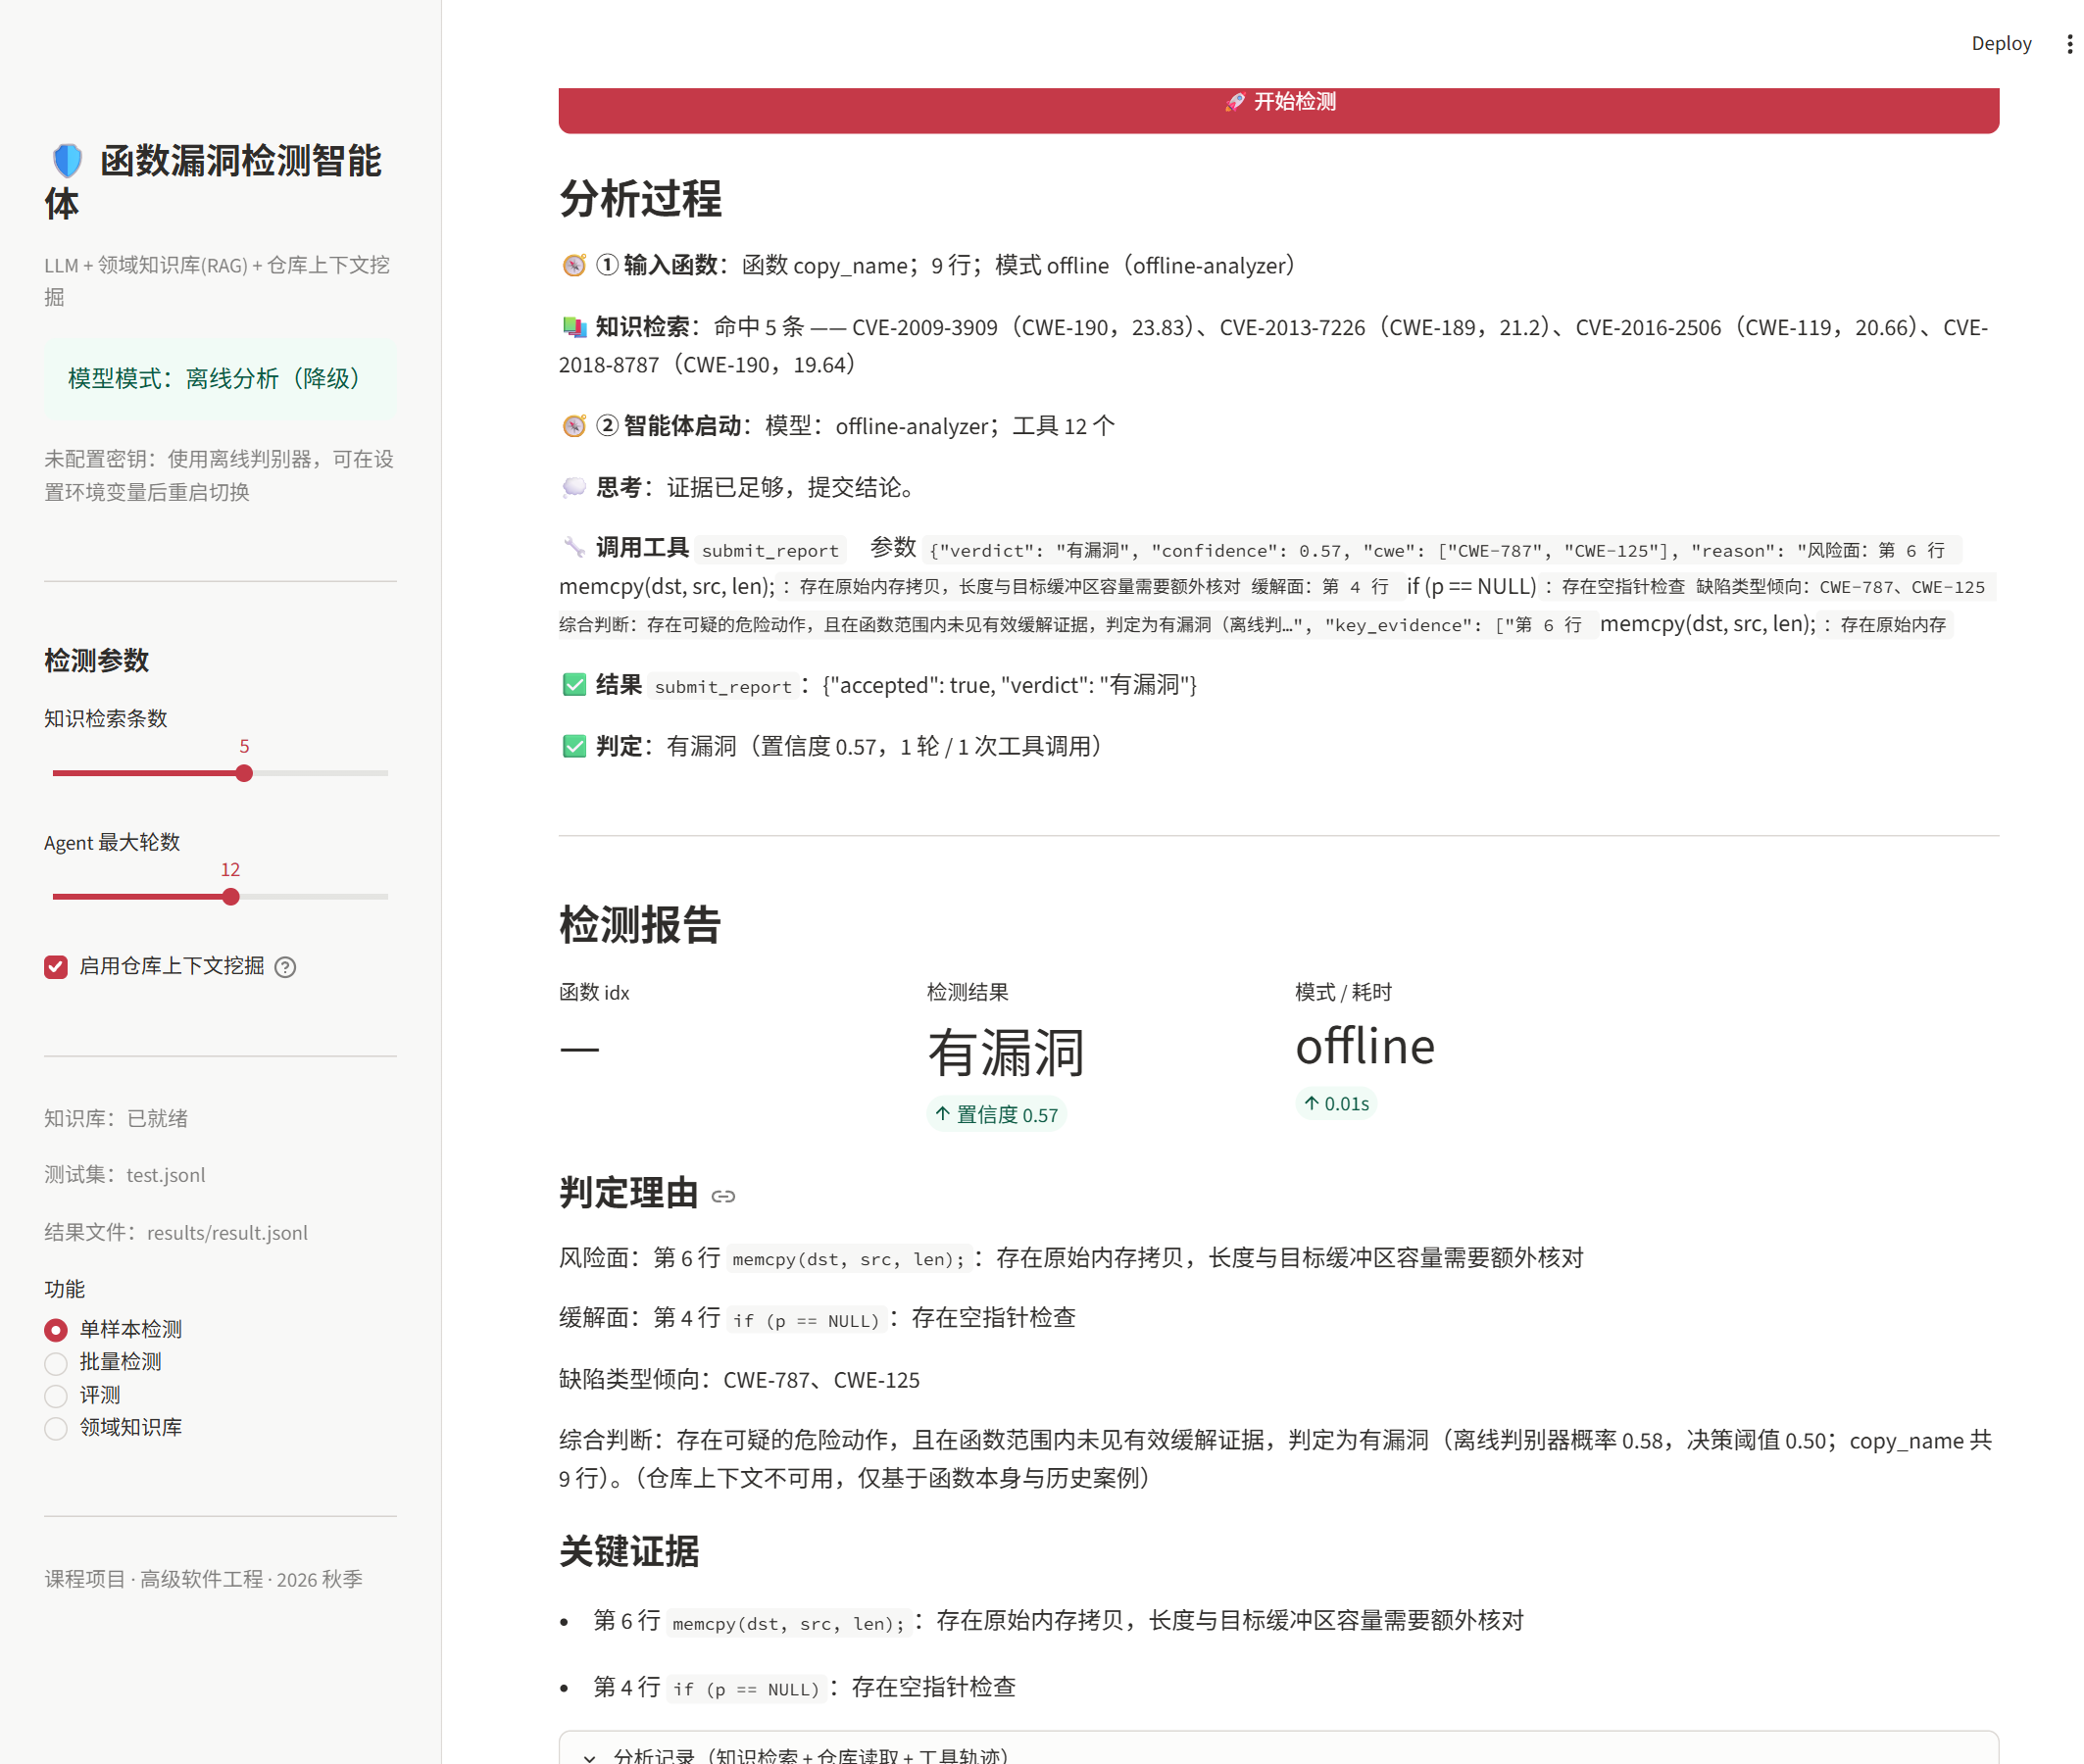
\includegraphics[height=4.5cm]{assets/shots/shot_report.png}\\[0.2em]
{\tiny \textbf{单样本检测}：左侧参数、右侧实时过程、下方四项报告}
\end{column}
\begin{column}{0.47\textwidth}
\centering
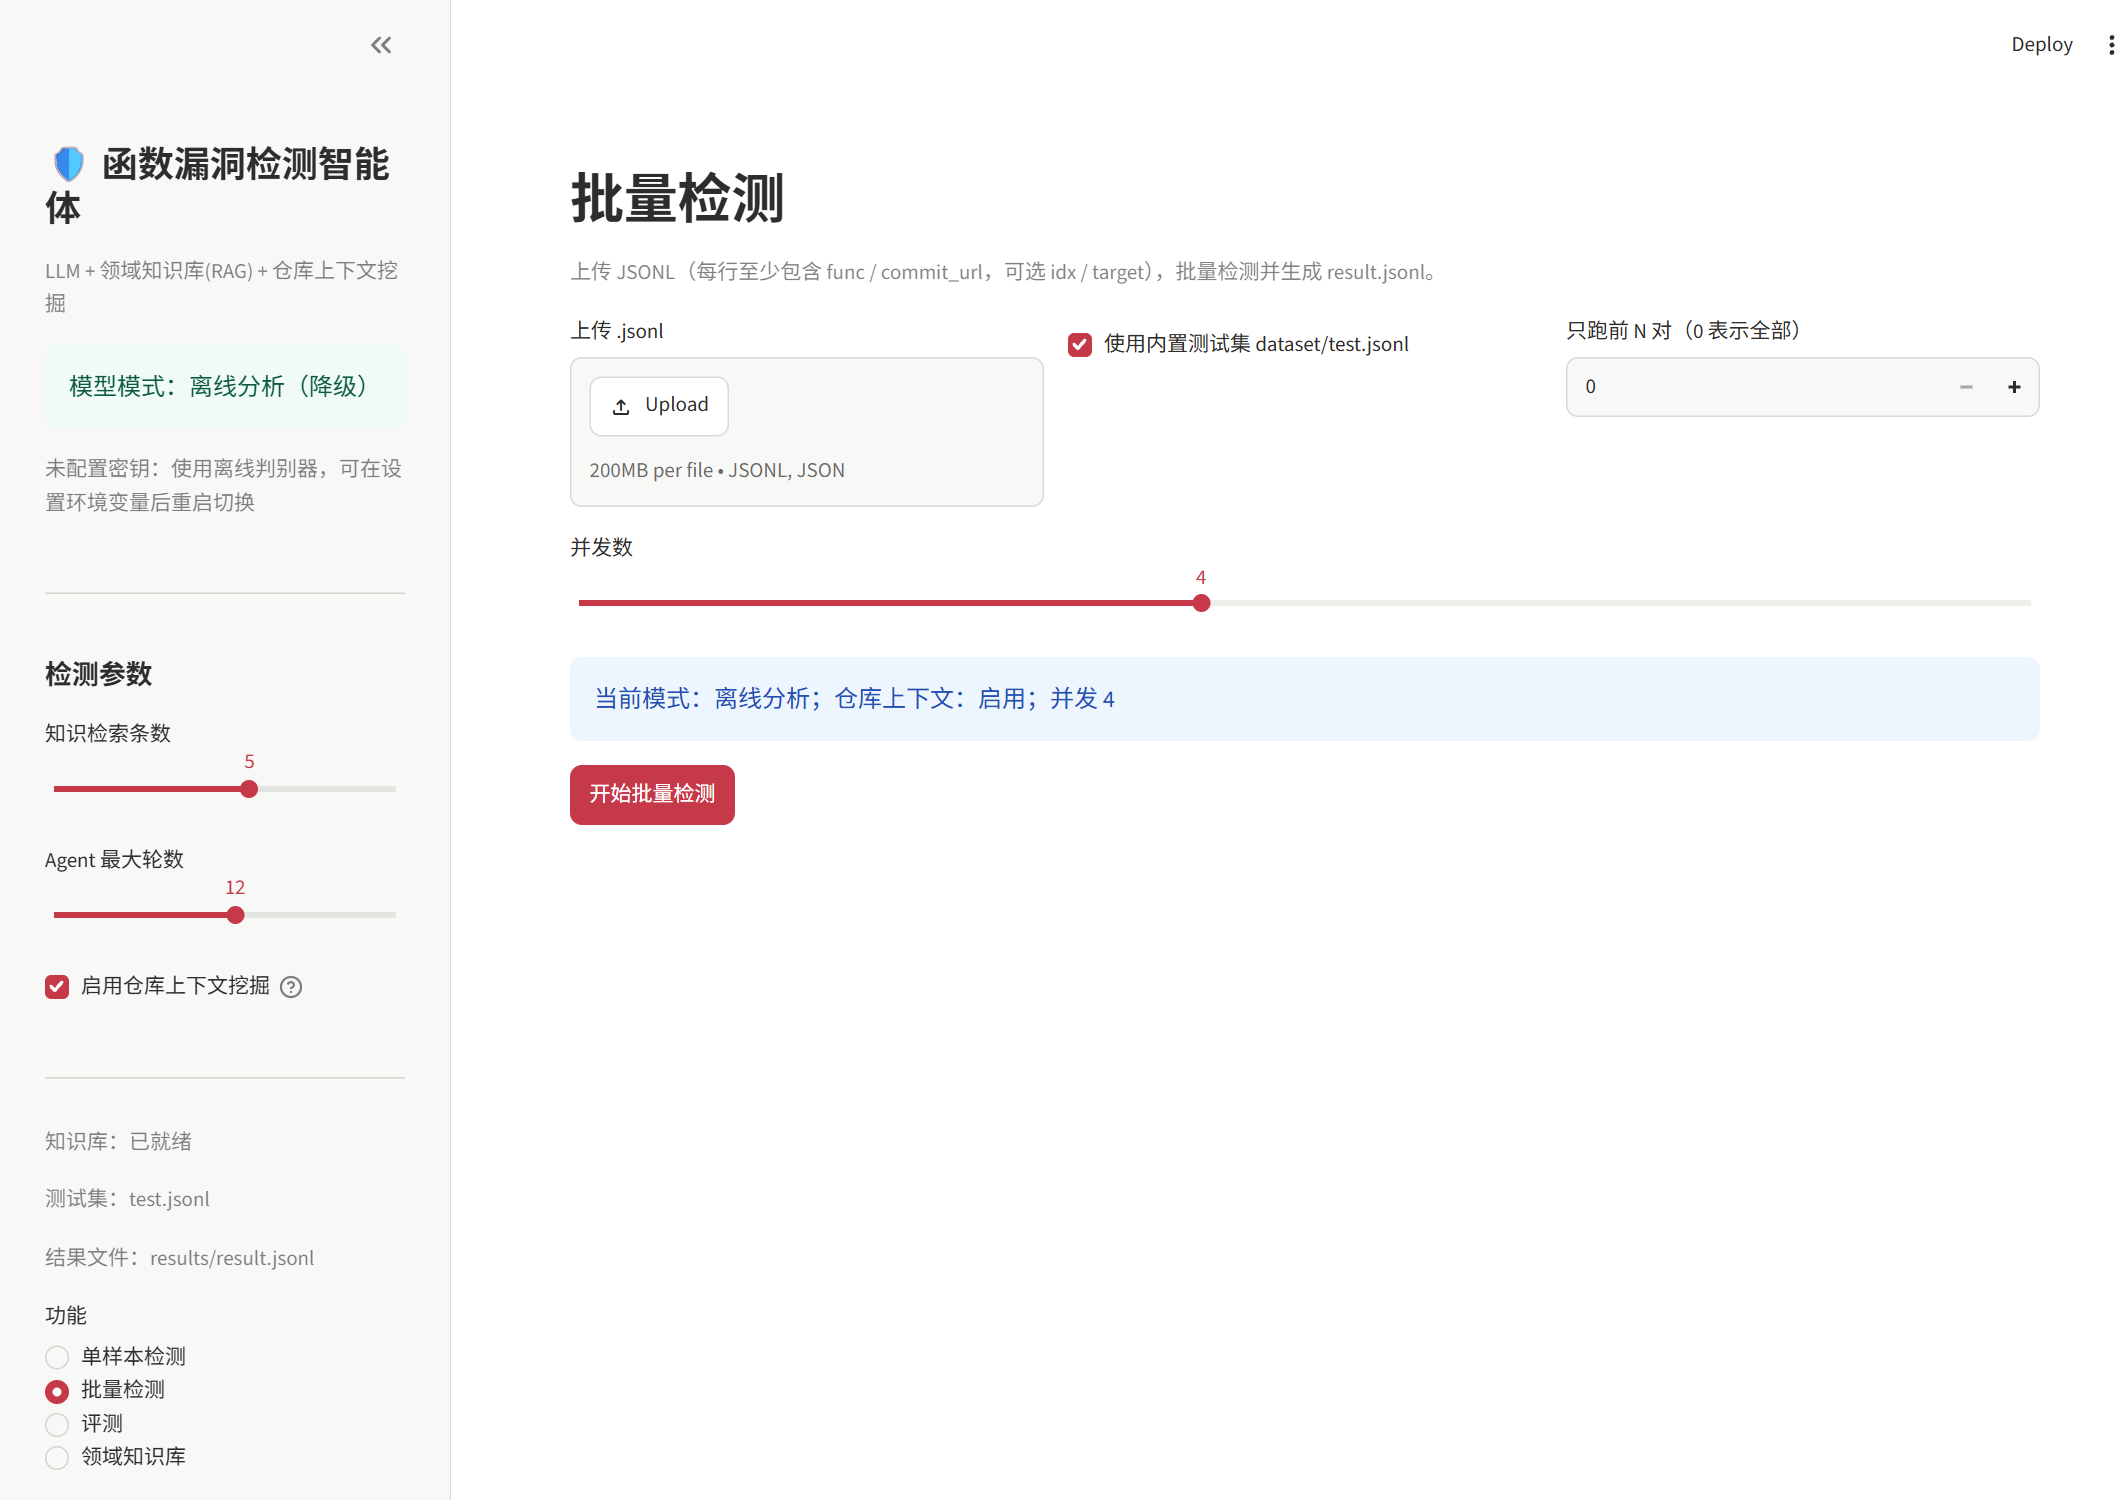
\includegraphics[height=4.5cm]{assets/shots/shot_batch.png}\\[0.2em]
{\tiny \textbf{批量检测}：上传 JSONL、进度、结果表与即时评测}
\end{column}
\end{columns}
\end{frame}

% ============================================================ 06 结果
\begin{frame}{06 · 评测结果：第一轮全量}
\framesubtitle{150 对样本、真实大模型 + 知识库 + 仓库取证}
\scriptsize
\begin{columns}[t]
\begin{column}{0.43\textwidth}
\begin{tabular}{@{}lrr@{}}
\toprule
\textbf{类别} & \textbf{组数} & \textbf{占比} \\
\midrule
P-C\ 成对正确 & \textbf{28} & 18.7\% \\
P-V\ 均判有漏洞 & 87 & 58.0\% \\
P-B\ 均判无漏洞 & 19 & 12.7\% \\
P-R\ 完全反转 & 16 & 10.7\% \\
\midrule
合计 & 150 & 100\% \\
\bottomrule
\end{tabular}

\vspace{0.5em}
\begin{colorblock}[black]{sintefyellow}{等级：C}
\tiny
P-C = 28 本应落在 B 档（25--29）；\\
但 P-R（16）$>$ P-C/2（14），触发课程降级规则，降为 \textbf{C}。\\
下一步核心目标：减少判反、减少两版判同。
\end{colorblock}
\end{column}
\begin{column}{0.55\textwidth}
\centering
\begin{tikzpicture}[x=0.052cm, y=1cm, font=\tiny]
% 堆叠条形图：总宽 150 单位
\draw[fill=sintefgreen]  (0,0)     rectangle (28,0.42);
\draw[fill=sintefyellow] (28,0)    rectangle (115,0.42);
\draw[fill=sintefgrey]   (115,0)   rectangle (134,0.42);
\draw[fill=sinteflilla]  (134,0)   rectangle (150,0.42);
\node[above] at (14,0.46)  {P-C 28};
\node[above] at (71.5,0.46){P-V 87};
\node[above] at (124.5,0.46){P-B 19};
\node[above] at (142,0.46) {P-R 16};
\draw[thick] (0,0) rectangle (150,0.42);
\end{tikzpicture}

\vspace{1.1em}
\begin{tabular}{@{}lrl@{}}
\toprule
\textbf{对照条件} & \textbf{P-C} & \textbf{等级} \\
\midrule
全判「有漏洞」/「无漏洞」 & 0 & D \\
离线判别器（无 LLM） & 9（6.0\%） & D \\
大模型 + 知识库（抽样 25 对） & 5（20.0\%） & --- \\
\textbf{完整 Agent（本轮全量）} & \textbf{28（18.7\%）} & \textbf{C} \\
\bottomrule
\end{tabular}

\vspace{0.4em}
{\tiny 相比无 LLM 的离线基线，成对正确数提升 \textbf{3.1 倍}。}
\end{column}
\end{columns}
\end{frame}

% ============================================================ 06 分析
\begin{frame}{06 · 结果分析：问题出在哪}
\framesubtitle{不是「判不出来」，而是「判得太保守」}
\footnotesize
\begin{columns}[t]
\begin{column}{0.47\textwidth}
\begin{colorblock}[black]{sinteflightgreen}{按函数规模看 P-C}
\scriptsize
\begin{tabular}{@{}lrr@{}}
\toprule
\textbf{规模} & \textbf{对数} & \textbf{P-C 率} \\
\midrule
$<$1k 字符 & 24 & 41.7\% \\
1k--3k & 55 & 16.4\% \\
3k--10k & 54 & 9.3\% \\
$>$10k & 17 & 23.5\% \\
\bottomrule
\end{tabular}\\[0.4em]
函数越长，模型越倾向于「看到可疑点就报」——
真正难的是\textbf{在长函数里确认某个可疑点已经被校验}。
\end{colorblock}
\end{column}
\begin{column}{0.49\textwidth}
\begin{colorblock}[black]{sinteflilla}{三个量化事实}
\scriptsize
\bad\ \textbf{过度报警}：300 条里 218 条被判「有漏洞」（72.7\%），
导致 P-V 占 58\%——修复版被反复误报。\\[0.3em]
\warn\ \textbf{判反 16 对}：主要发生在「修复版里有新增校验、但漏洞版也有类似写法」的函数上。\\[0.3em]
\good\ \textbf{长尾有效}：小函数 P-C 41.7\%，说明语义判断链路本身是通 的，
问题集中在「边界条件」与「长上下文」。
\end{colorblock}
\end{column}
\end{columns}

\vspace{0.3em}
\begin{center}
\footnotesize
按仓库：TensorFlow（69 对）P-C 11 对；GPAC（16 对）3 对；mruby（6 对）2 对；
而本测试集有 \alert{49\%} 的样本来自 TensorFlow / Linux——这些仓库的快照被体量守卫跳过，
Agent 只能靠函数本身与历史案例判断。
\end{center}
\end{frame}

% ============================================================ 07 创新点
\begin{frame}{07 · 创新点与特色}
\framesubtitle{围绕「可解释、可复核、可复现」做工程取舍}
\footnotesize
\begin{columns}[t]
\begin{column}{0.48\textwidth}
\begin{colorblock}[black]{sinteflightgreen}{方法与设计}
\scriptsize
\good\ \textbf{成对案例 + 修复要点}：把「当年怎么修的」提炼成可检索先验，
而不是只索引单个函数。\\[0.25em]
\good\ \textbf{证据驱动而非固定流水线}：工具集合固定、调用顺序由模型决定，
配合预算与收敛策略，避免「无脑全仓扫描」。\\[0.25em]
\good\ \textbf{严格版本隔离可审计}：父提交 / 提交后二选一，无 diff、提示词不含标签。\\[0.25em]
\good\ \textbf{过程留痕}：每次检索与读取都产生事件流，报告可回放到每一步。
\end{colorblock}
\end{column}
\begin{column}{0.48\textwidth}
\begin{colorblock}[black]{sintefyellow}{工程特色}
\scriptsize
\good\ \textbf{零依赖核心}：BM25 + 自研解析 + 自研 ReAct，换机器不必重装生态。\\[0.25em]
\good\ \textbf{成本守卫}：仓库体量超 300 MB 自动跳过并如实标注，
避免被 TensorFlow 这类仓库拖垮整批评测。\\[0.25em]
\good\ \textbf{无密钥也能跑}：离线降级模式保证演示与回归测试始终可用，
同时充当消融基线。\\[0.25em]
\good\ \textbf{一键复现}：三个 \texttt{.bat} + 31 项自动化测试，
从零到出分只需两条命令。
\end{colorblock}
\end{column}
\end{columns}
\end{frame}

% ============================================================ 08 问题与计划
\begin{frame}{08 · 当前存在的问题}
\framesubtitle{四个待解问题，按影响大小排序}
\scriptsize
\begin{tabular}{@{}p{0.04\textwidth}p{0.25\textwidth}p{0.38\textwidth}p{0.22\textwidth}@{}}
\toprule
 & \textbf{问题} & \textbf{证据} & \textbf{影响} \\
\midrule
1 & 判定过度保守，修复版被误报 & P-V 87 对（58\%）；300 条中 218 条判「有漏洞」 & 直接压低 P-C \\
\addlinespace[1pt]
2 & 方向性错误（判反） & P-R 16 对（10.7\%）$>$ P-C/2，触发降级 & 等级从 B 掉到 C \\
\addlinespace[1pt]
3 & 长函数上准确性骤降 & 3k--10k 字符区间 P-C 仅 9.3\% & 覆盖率最高区间反而最弱 \\
\addlinespace[1pt]
4 & 仓库上下文覆盖不足 & 49\% 样本来自超大仓库，快照被体量守卫跳过 & 最强的证据用不上 \\
\bottomrule
\end{tabular}

\vspace{0.5em}
{\scriptsize \textbf{根因判断}：提示词把「有可疑点」与「有漏洞」绑得太紧——缺少
「\textbf{必须证明这个可疑点在当前代码中确实没有被缓解}」的强制步骤；
加上长函数超出单次观察上限，模型只能保守报警。}
\end{frame}

% ============================================================ 08 下一步
\begin{frame}{08 · 下一步优化计划}
\framesubtitle{每条措施都对应一个可验收指标}
\tiny
\begin{tabular}{@{}p{0.22\textwidth}p{0.46\textwidth}p{0.26\textwidth}@{}}
\toprule
\textbf{优化方向} & \textbf{具体做法} & \textbf{验收指标} \\
\midrule
抑制过度报警 & 两阶段判定：先列可疑点，再单独一轮「找缓解证据」；
提示词要求「未被缓解」必须给出反证 & P-V 从 58\% 降到 45\% 以下 \\
\addlinespace[1pt]
减少判反 & 引入「修复形态比对」：把当前代码与历史案例的修复要点逐条对照，
强制模型解释「为什么这个修复已存在 / 不存在」 & P-R 降到 10 对以内 \\
\addlinespace[1pt]
长函数处理 & 函数切片：按危险操作定位片段 + 调用关系图，分批送入模型；
超长函数先摘要再精读 & 3k--10k 区间 P-C $\geq$ 25\% \\
\addlinespace[1pt]
仓库取证 & 只取相关文件：GitHub Tree API + 按需 blob；增量快照与共享缓存
& TensorFlow 样本可取证比例 $>$ 50\% \\
\addlinespace[1pt]
评测与复现 & 全量 300 条用完整 Agent 模式复跑；做「有 / 无仓库上下文」的消融对比
& 给出置信区间与消融表 \\
\bottomrule
\end{tabular}

\vspace{0.5em}
{\scriptsize \textbf{时间安排}：W6 完成「两阶段判定 + 修复形态比对」并复跑全量；
W7 补齐消融实验与技术报告、准备现场演示。目标等级 \textbf{B 及以上}。}
\end{frame}

% ============================================================ 结尾
\begin{frame}{谢谢，请老师和同学批评指正}
\framesubtitle{现场演示：单样本检测 → 分析记录 → 批量评测}
\vspace{0.2em}
\begin{columns}[t]
\begin{column}{0.48\textwidth}
\begin{colorblock}[black]{sinteflightgreen}{本次汇报要点}
\scriptsize
\good\ 六项功能全部落地，可现场演示完整流程\\
\good\ 真实模型全量评测：P-C 28 / 150，等级 C\\
\good\ 已定位「过度报警、判反、长函数、快照成本」四个问题\\
\good\ 下一步措施与验收指标已明确
\end{colorblock}
\end{column}
\begin{column}{0.48\textwidth}
\begin{colorblock}[black]{sintefyellow}{代码与文档}
\scriptsize
\textbf{代码}：\texttt{github.com/LiLisyn123/func-vuln-agent}\\[0.2em]
\textbf{文档}：\texttt{README.md}、\texttt{使用教程.md}、\\
\quad\texttt{docs/项目报告.md}\\[0.2em]
\textbf{复现}：\texttt{batch} $\rightarrow$ \texttt{eval}
\end{colorblock}
\end{column}
\end{columns}
\end{frame}

\end{document}
